%Signal quality assessment is a fundamental component in the area of health monitoring applications, especially in the context of health applications in wearable devices%~\cite{lucafo2022}. These wearable devices serve as instruments for the continuous measurement of vital signs and health parameters, yet their efficacy is contingent upon the rigorous evaluation of the signals they capture. Although those devices are usually designed for long periods of monitoring, they use an optical method to obtain a \acrfull{ppg}, signal type that may deteriorate due to many factors, including motion artifacts or changes in illumination, thereby requiring signal quality assessment mechanisms to check its reliability. The quality of the data derived from these devices plays a decisive function in the efficacy of machine learning and artificial intelligence algorithms, frequently deployed for health data analysis and decision-making. Thus, by ensuring signal quality, wearable health applications can mitigate false alarms, deliver tailored healthcare recommendations, bolster research endeavors, and enhance device adoption and long-term utilization, consequently advancing the landscape of healthcare and patient well-being. In this work, we propose a solution for the problem of assessing the quality of 1D %\acrshort{ppg} signals by projecting them into 2D images, to take advantage of %\gls{CV} techniques, which requires bi-dimensional data.

The human civilization constantly seeks improvements in life longevity and quality. One of the main research areas in that regard is the medicine, which provides means of preventing and remedying accidents and diseases. Diseases, specifically, can deteriorate a person's health silently. An example of that is the presence of atheromas, which, when untreated, can lead to lethal events such as heart attacks and strokes. For that reason, it is important to periodically search professional medical advice to detect diseases at early stages when it is still easy to treat them. However, individual professional service is expensive for most people and is unresponsive to sudden changes. Therefore, there is a demand for an automatic and constant health monitoring method.  

A promising solution for that demand is the continuous healthcare monitor applications enabled by wearables. That approach is particularly possible due to the advent of \gls{IoT}, which is, in concept, a scalable network of interconnected devices that exchange information possibly acquired by sensors \cite{aouedi2024survey}. It is interesting for healthcare when those sensors extract environmental and physiological data that can hint the patient conditions. Examples of such data are body temperature, blood pressure and neural activity. We can obtain those indicators in the patient daily life through wearable devices that resemble quotidian objects, with the shape of belts, bracelets, rings, shoe soles, clothing, etc \cite{van2024smart}. An popular example of such wearables is the smartwatches that, similarly to smartphones, can execute multiple applications, such as recording physiological data. Since devices like those support wireless connection, they can send that data to either directly to a medical staff or, as the now popular big data trend promotes, to an automatic intelligent system in the cloud. That intelligent system can, among countless patients, choose special cases that need attention. Therefore, the remote healthcare promises easier than ever access to key physiological signal data. 

Despite the advantages of continuous health monitoring using smart wearables, the extraction of physiological signals is not free of interferences. \gls{PPG} signals, for instance, is under the influence of changes in illumination, low sensor quality, user skin physiognomy, adverse sensor positioning, etc. These influences can impair the signal to the point that its use becomes unfeasible. Moreover, \gls{PPG} signals are highly susceptible to artifacts generated by motion or noise sources. For instance, wrist movements can disrupt the signal in a smartwatch \gls{PPG} sensor, though the degree of distortion varies with the signal power and wavelength. These variation can cause high-amplitude distortions that not only can destroy the core information, but can also produce misleading events. These events are unacceptable in healthcare applications since misdiagnosis can expose the healthy patient to unnecessary risk, while lack of diagnosis can leave the unhealthy patient unattended. For that reason, it is of extreme importance to verify the quality of the signal before proceeding to further analysis on the signal. That task is known as \gls{SQA} and this thesis proposes a method to achieve that goal for \gls{PPG} signals.


\section{Problem Description}
\label{sec:problem}

Traditionally, the two most frequently used methods for evaluating the cardiac cycle and monitoring heart rate are \glsfirst{ECG} and \glsfirst{PPG}. The \gls{ECG} has long been considered the gold standard for detecting heart rate and diagnosing cardiovascular conditions. It monitors the electrical impulses responsible for heart muscle contractions through electrodes attached to the body, usually positioned on the chest. Although \gls{ECG} is the mainstay for cardiac assessments, it is not typically suitable for long-term monitoring or challenging environments due to its intricate data collection process. Conversely, \gls{PPG} offers a more practical approach for observing cardiorespiratory metrics. It employs compact optical sensors and a light source to detect variations in skin color caused by blood flow following each heartbeat. The \gls{PPG} measures the blood flow rate in tissues (e.g., wrist), influenced by the heart's pumping action, making it particularly effective for peripheral circulation monitoring, especially with wrist-worn or finger-mounted devices.

\begin{figure}[h!]
	\centering
	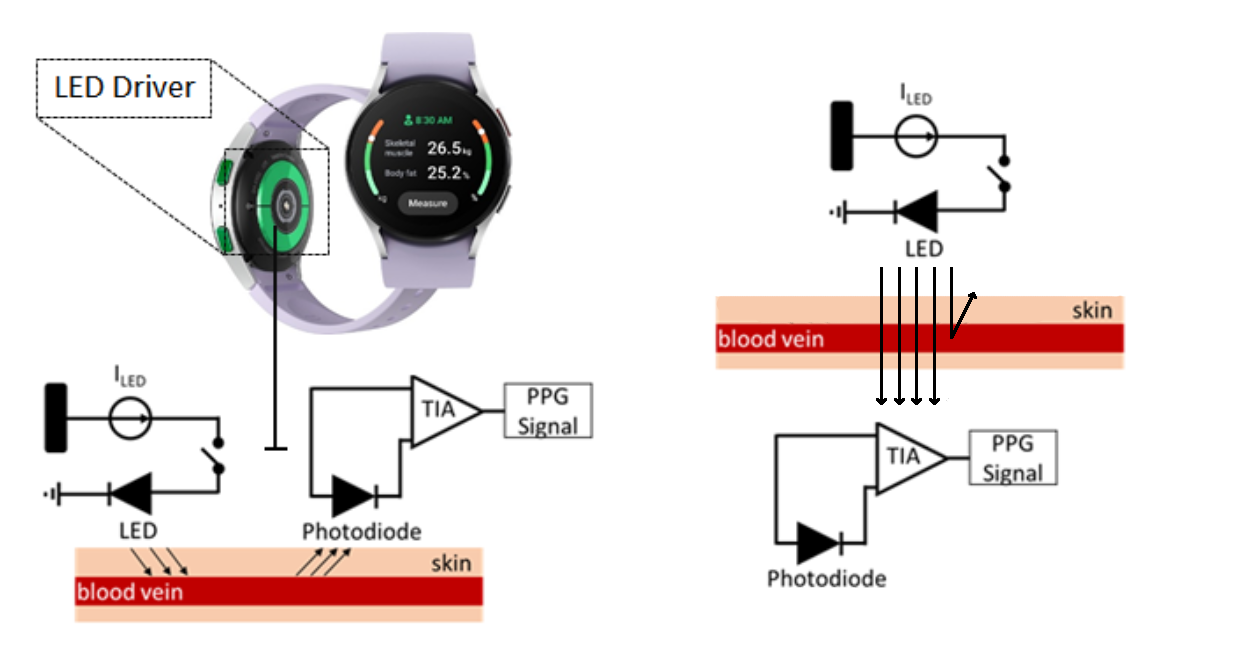
\includegraphics[width=0.9\textwidth]{img/ppg.png}
	\caption{Schematic illustration of a \gls{PPG} sensor. On the left, the signal is obtained through the reflectivity of light by human tissue, while on the right, it is obtained through the permeability of light through human tissue. This figure is a courtesy of Lucafó et al.~\protect\cite{deep-learning-3}}
	\label{fig:method:ppg}
\end{figure}


In more detail, \gls{PPG} signals are optical signals that result from the interaction of light with human tissue. To extract the signal, two basic components are needed. The first is a light source, which emits light towards the tissue. An example of a light source is the \gls{LED}. The second component is a light receptor, which measures the light intensity. While a photodiode is commonly used for this purpose, cameras have also been employed. For signal extraction, these two types of devices are positioned to exploit one of two light interaction principles. Figure~\ref{fig:method:ppg} illustrates both principles. The first principle is light reflectance, where human tissue reflects incoming light rays. In this case, the devices should be positioned so that the tissue is not between them. An example of this application is smartwatches, where all devices are positioned below the main structure. The second principle is light permeability, where light can traverse the human tissue. Here, the devices should be placed such that the tissue is between them. An example of this setup is fingertip pulse oximeters. Once the setup is complete, the \gls{PPG} signal can be extracted.

\begin{figure}[h!]
    \centering
    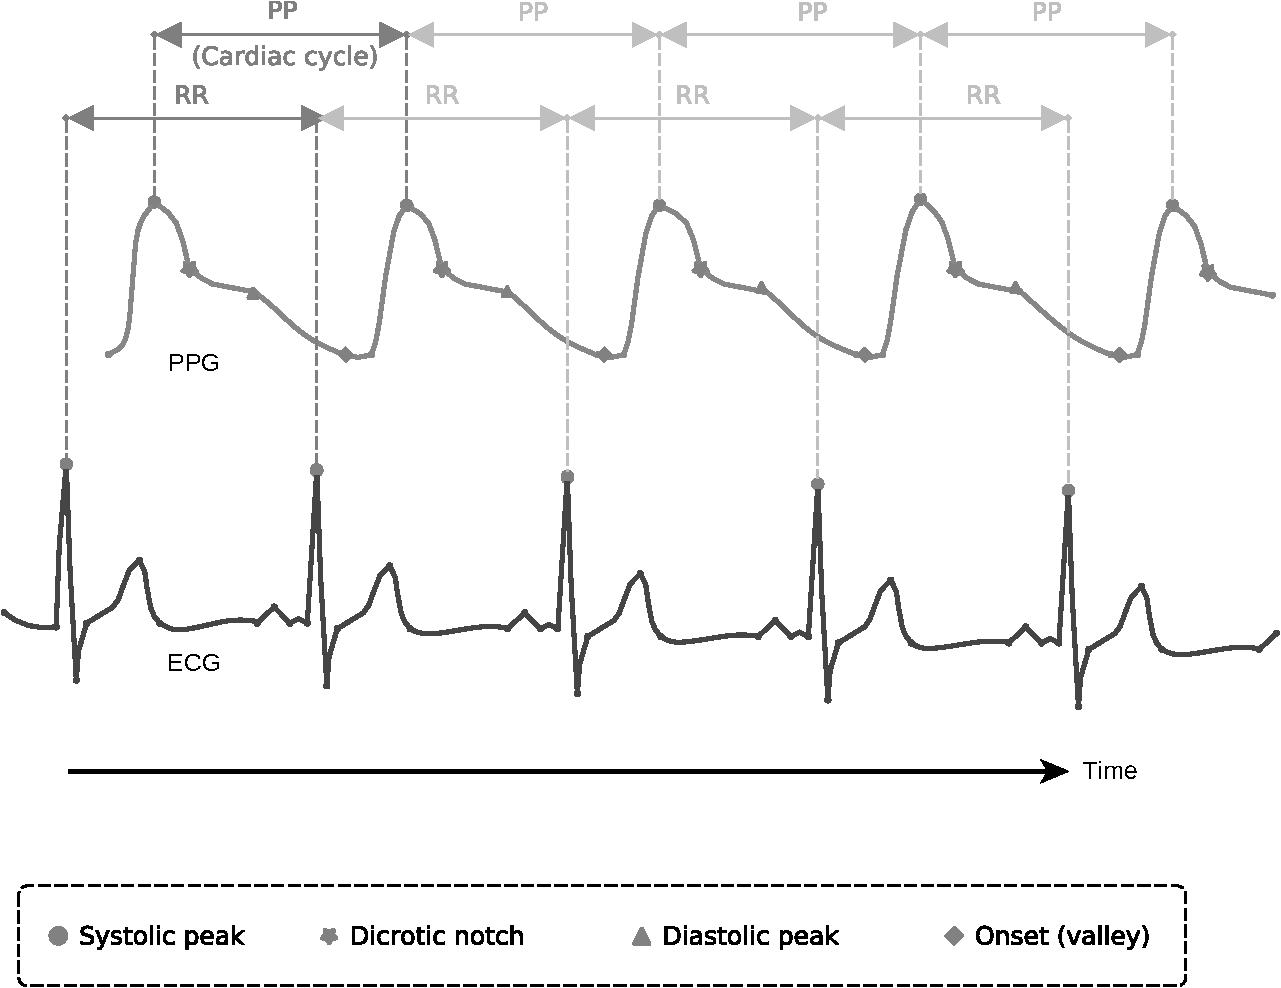
\includegraphics[width=0.75\textwidth]{img/ecg_ppg_signals.pdf}
    \caption{Inter-Beat Interval (IBI) estimation using RR Interval from Electrocardiogram (ECG) and the corresponding Peak-to-Peak Interval from Photoplethysmography (PPG).}
    \label{fig:ecg_and_ppg}
\end{figure}


Since both \gls{ECG} and \gls{PPG} gauge cardiovascular and circulatory parameters, they are interconnected, as depicted in Figure~\ref{fig:ecg_and_ppg}. The similarity in the signal periods of both methods suggests that either can be used to analyze metrics such as the \gls{IBI}. Additionally, Figure~\ref{fig:ecg_and_ppg} emphasizes the reference points often utilized to assess health indicators related to blood pressure, oxygen saturation, and more.


\begin{figure}[h!]
    {
    \def\arraystretch{1}
    \setlength{\tabcolsep}{2pt}
    \begin{tabular}{cc}
        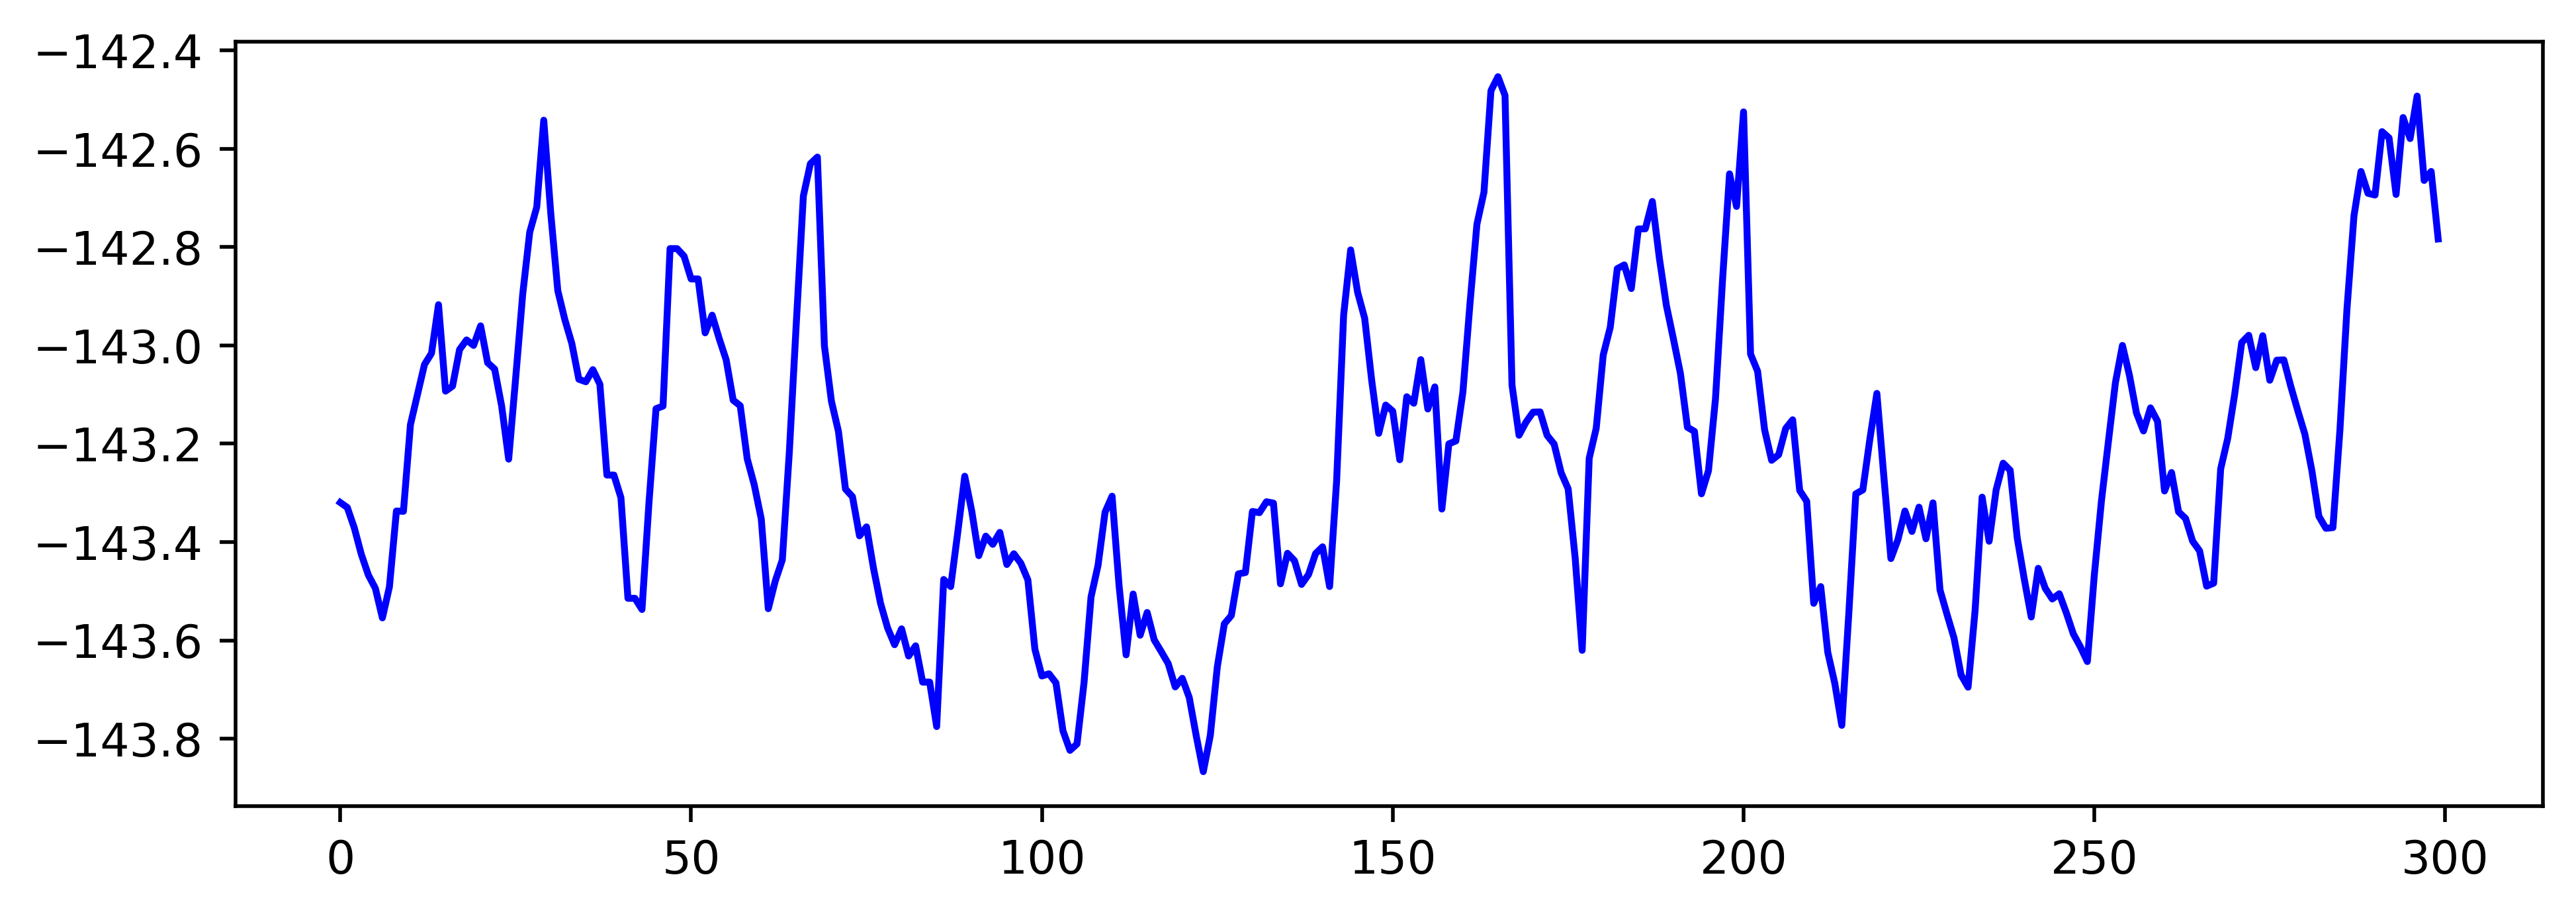
\includegraphics[width=0.48\textwidth, trim={1.5em 0 0em 0}, clip]{img/samples/butppg_111001.png} 
        & 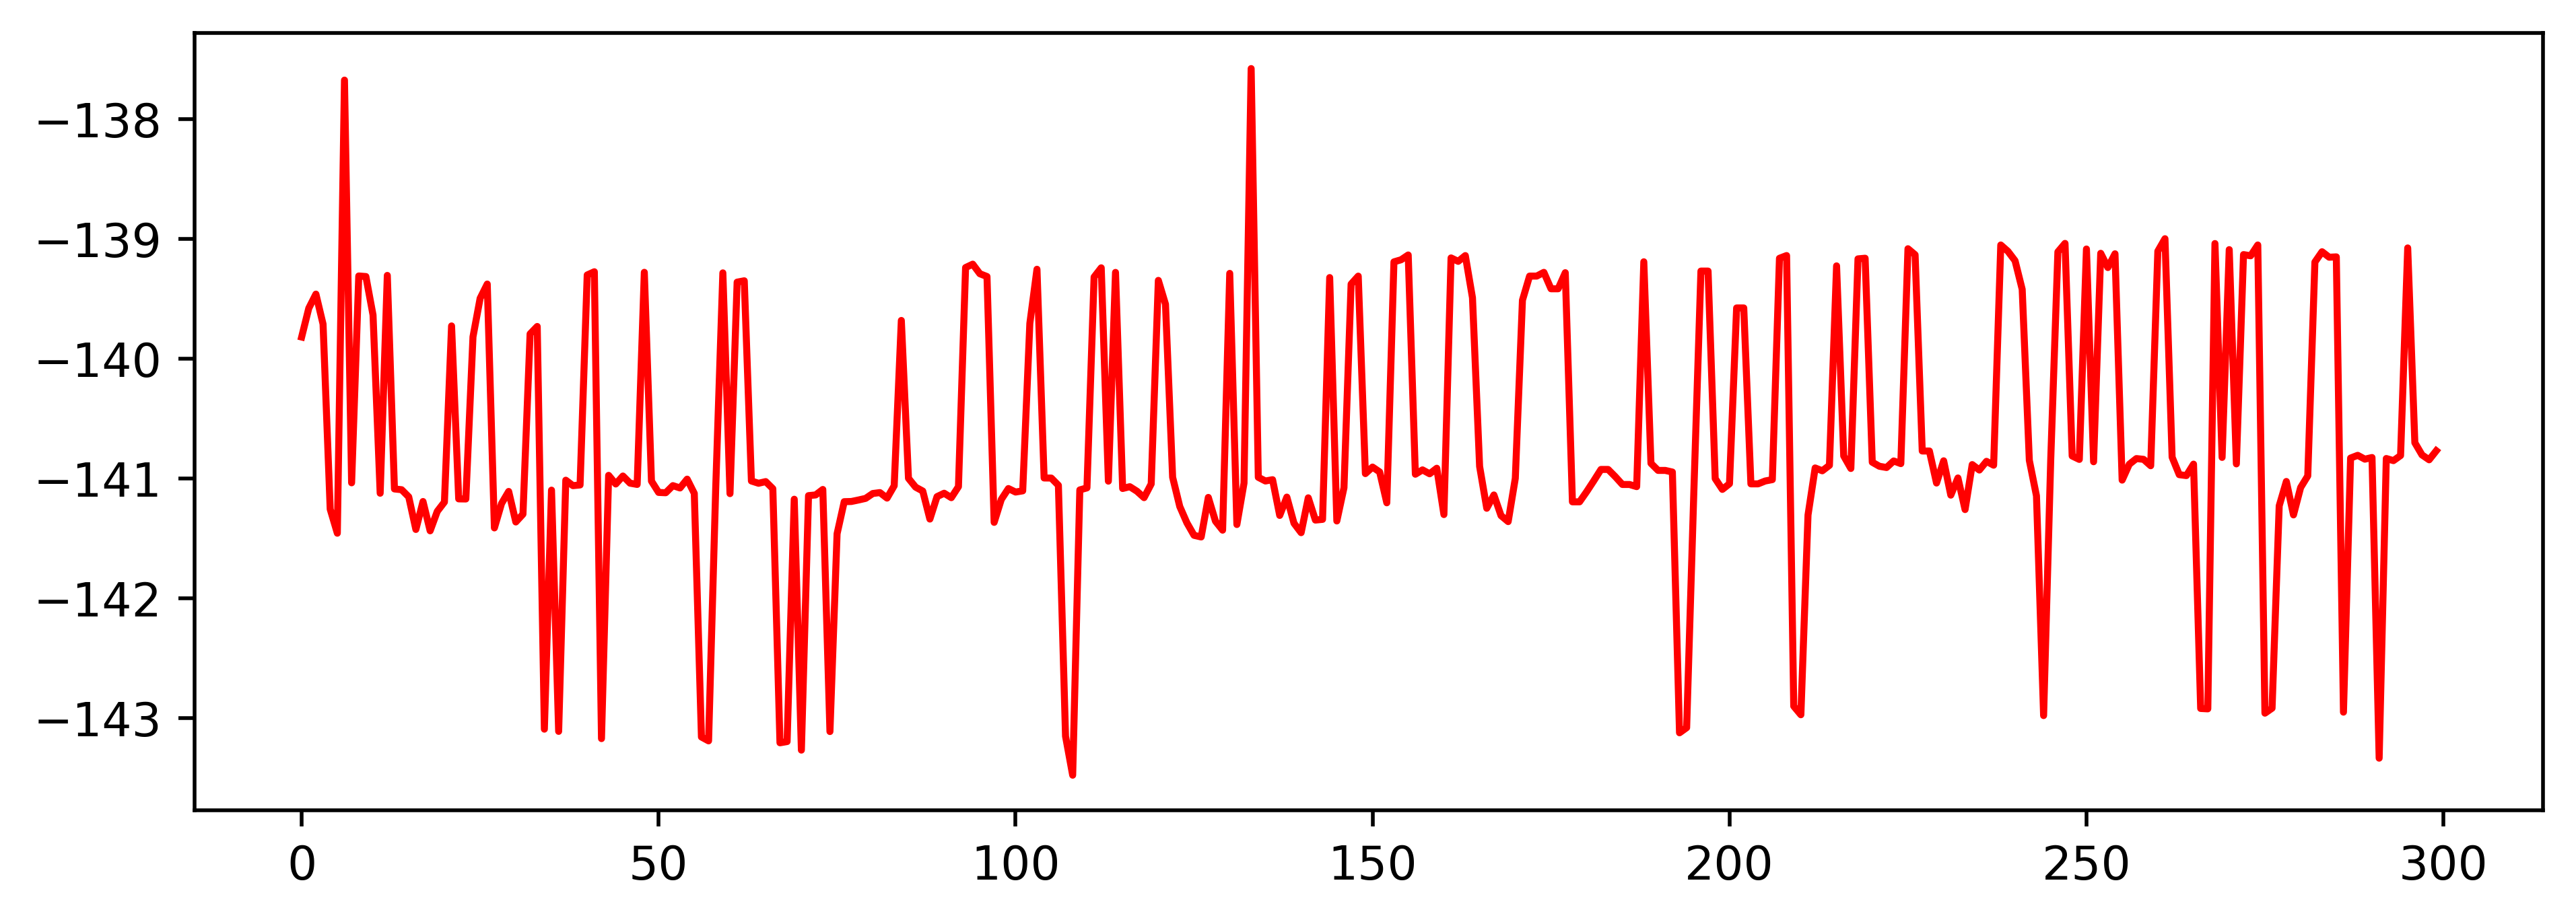
\includegraphics[width=0.48\textwidth, trim={1.5em 0 0em 0}, clip]{img/samples/butppg_111003.png} \\
        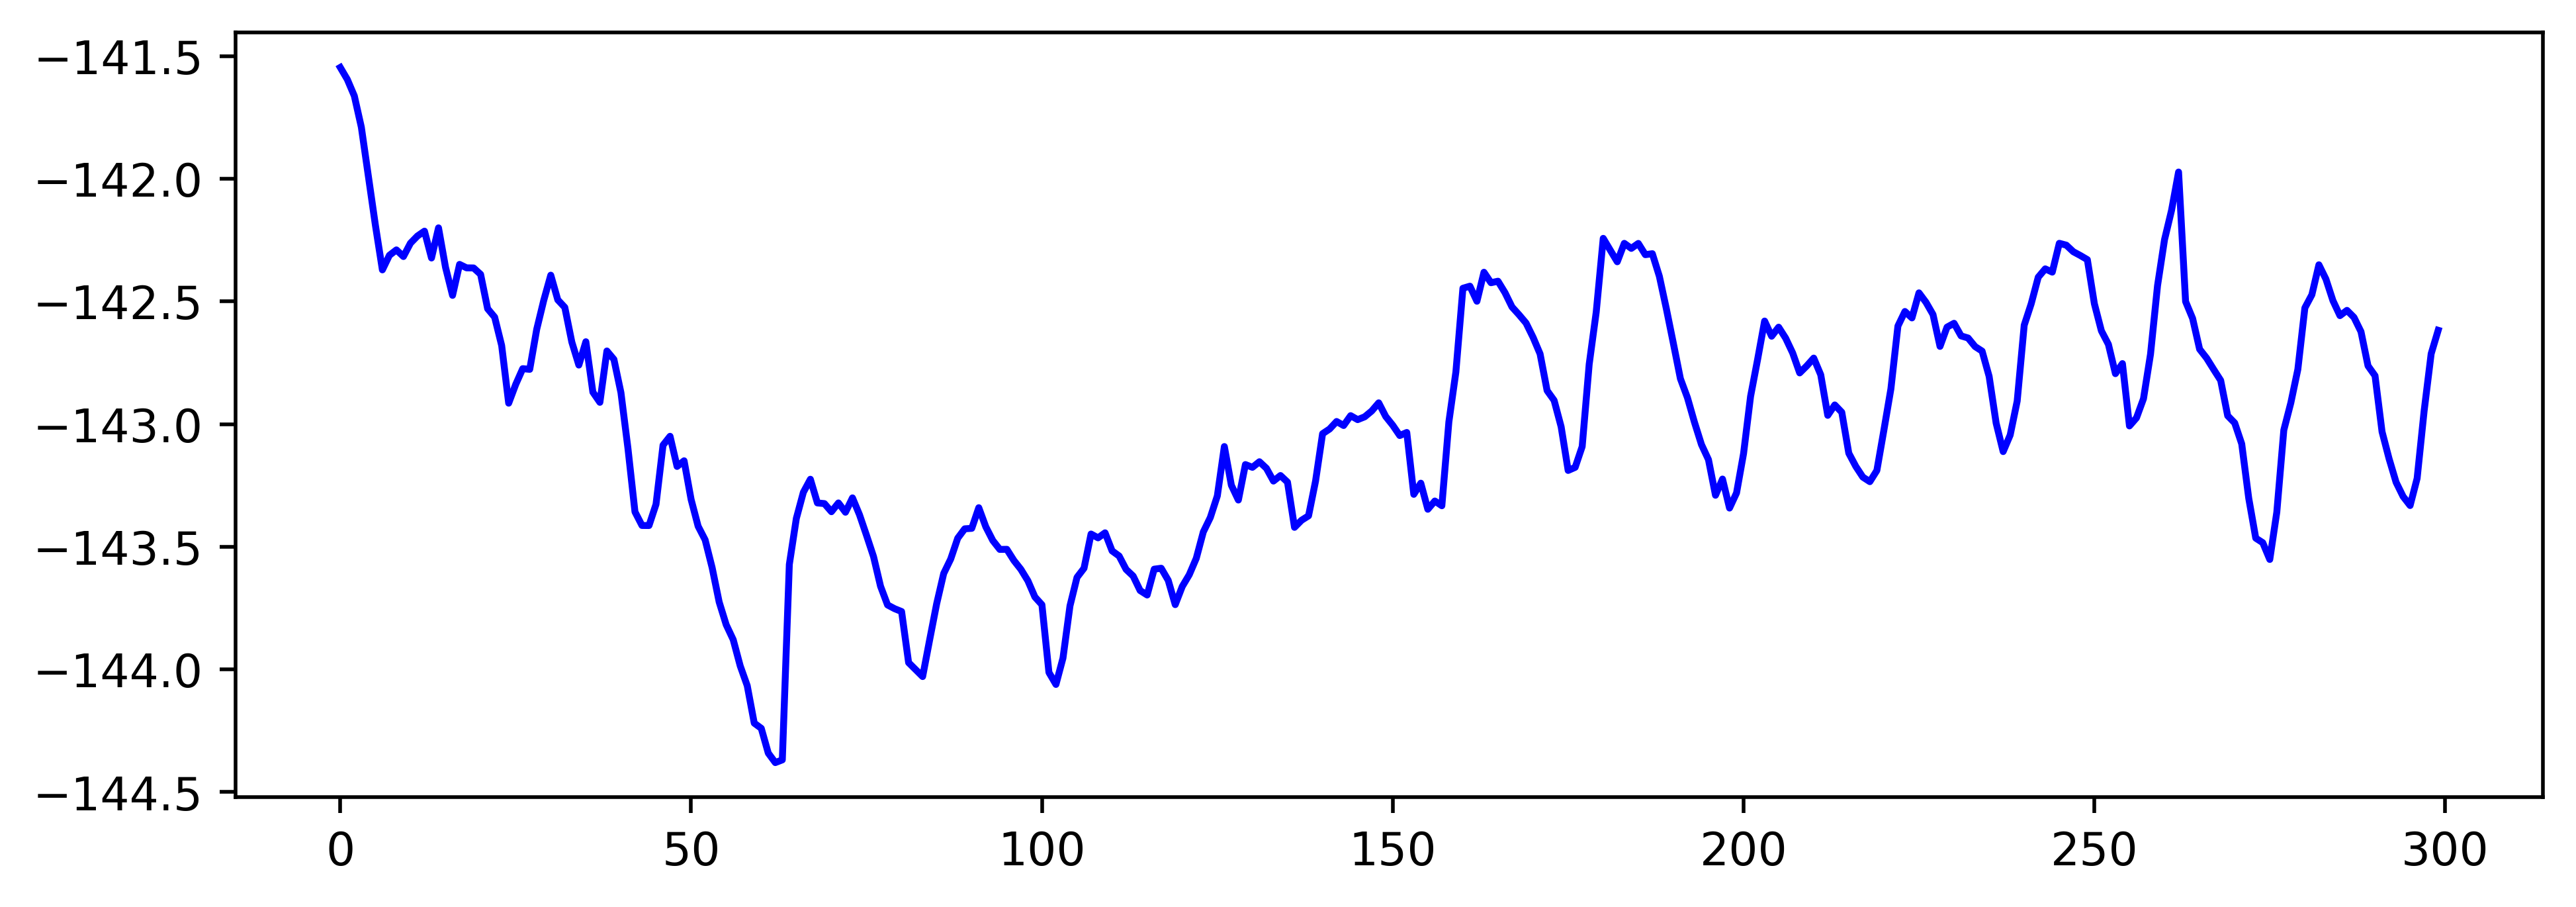
\includegraphics[width=0.49\textwidth, trim={1.5em 0 0em 0}, clip]{img/samples/butppg_111002.png} 
        & 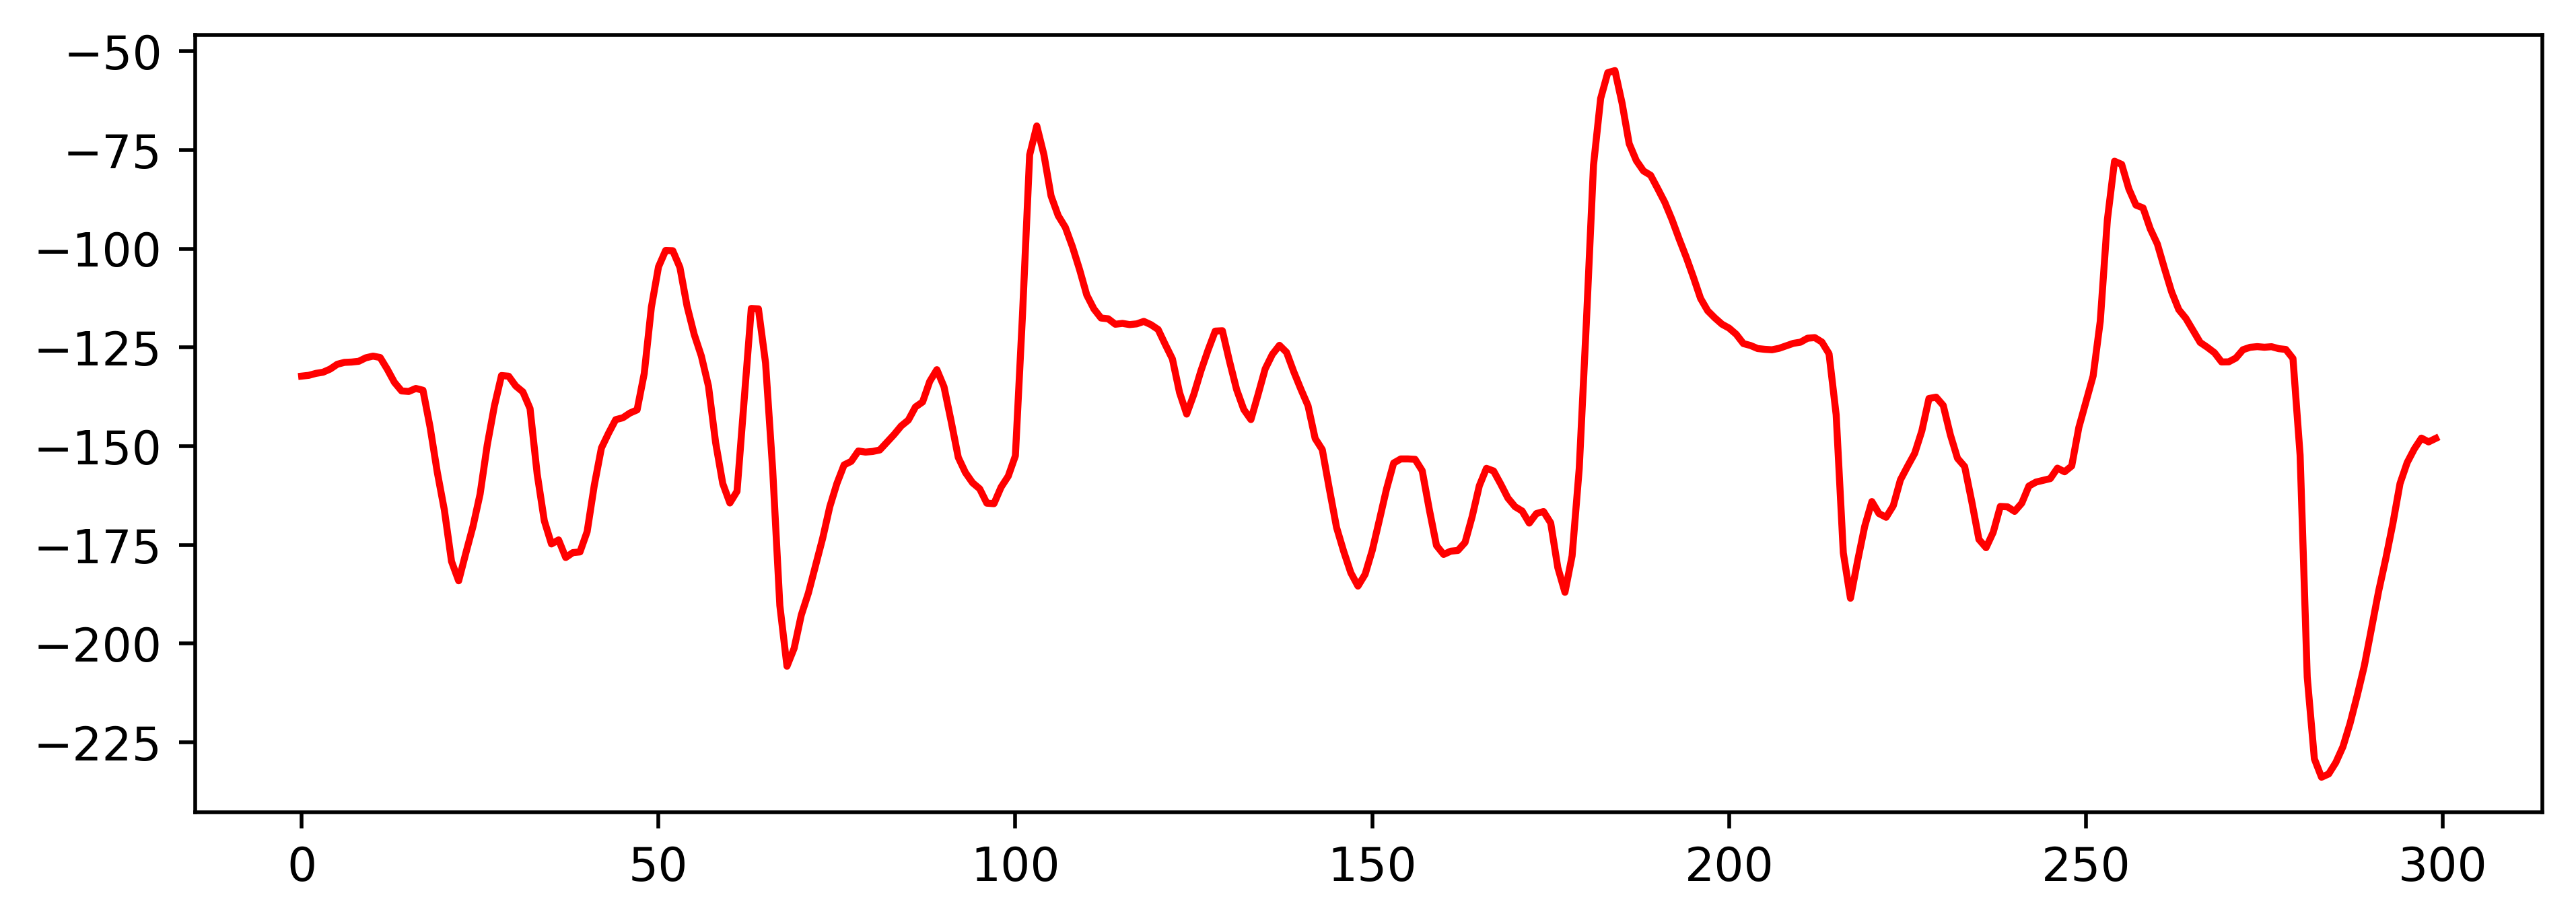
\includegraphics[width=0.49\textwidth, trim={1em 0 0em 0}, clip]{img/samples/butppg_111004.png} \\
    \end{tabular}
    }
    \caption{Example of 'good' (reliable) and 'bad' (unreliable) PPG signals. A `good' signal (blue) exhibits symmetrical, well-defined, and more consistent patterns. In contrast, `bad' signals (red) present irregular, asymmetrical patterns with reduced consistency and greater variability between periods. In these graphs, the vertical dimension is the average of all pixels intensity in a frame, while the horizontal dimension is the time instant in frames. These records are 10 seconds long and sampled with a frequency of 30 Hz. These signals were plotted using signals from BUTPPG~\protect\cite{butppg} database.}
    \label{fig:butppg_samples}
\end{figure}

Typically, \gls{PPG} signals are highly prone to degradation due to various factors, especially motion artifacts. Excessive movement of the \gls{PPG} sensor can cause significant distortion in the waveform, which affects the accuracy of subsequent signal analysis. These artifacts obscure or distort vital information within the signal. Figure~\ref{fig:butppg_samples} illustrates examples of both reliable and distorted \gls{PPG} signals. Distorted signals can lead to incorrect decisions and misclassification, which is unacceptable in health and wellness applications. As a result, methods for assessing \gls{PPG} signal quality are essential to prevent misinterpretation by differentiating between reliable and noisy data.

\section{Contributions of This Work}
\label{sec:my_work}

The main contributions of this thesis are the development of a quality assessment framework for \gls{PPG} signals. This framework is developed through several key contributions. Firstly, it proposes a new and effective approach for encoding time series into a set of 2D images. More specifically, the proposed method aggregates different projections into a composite hyperspectral image. This approach is based on the assumption that this aggregation provides better descriptiveness than using only a single projection. Additionally, this work evaluates the proposed approach in combination with a wide range of \gls{CV} models, which previous works have not done. This evaluation provides insights into which types of models are ideal for the time series matrix embedding technique. Thirdly, the thesis explores a novel idea of transfer learning using a dataset outside the \gls{SQA} domain, specifically the ImageNet dataset~\cite{ImageNet}. Finally, the thesis reports experiments conducted on a publicly available labeled dataset, named \gls{BUTPPG}~\cite{butppg}, which enhances the reproducibility and comparability of the experiments. The lack of reproducibility is a noticeable problem in the field currently, and the systematic empirical study conducted in this work can be useful for the community.

\section{Organization of This Thesis}
\label{sec:organization}

This Undergraduate thesis is organized in 5 chapters: this introduction; an overview of similar works existing in the literature; the proposed \gls{PPG} signal quality assessment method; simulation, results and comparisons; and conclusions. Chapter 2 contains an overview of the \gls{SQA} ecosystem and its quality assessment methods. Chapter 3 describes the proposed contributions of this thesis, containing all the proposed quality assessment methods. Chapter 4 contains the experimental setup, simulation results and comparisons of the proposed \gls{SQA} quality assessment methods and other state-of-the-art methods. Finally, Chapter 5 presents the conclusions of this work. 


